\documentclass{../kin_math}

\header{Elijah Kin}{Homework 10}{AMSC660}
\headrule

\begin{document}

\begin{questions}
  \question Suppose that a smooth function $f(x)$ is approximated by a quadratic model in the neighborhood of a current iterate $x$:
  \begin{equation*}
    m(p) = f(x) + \nabla f(x)^\top p + \frac{1}{2} p^\top B p,
  \end{equation*}
  where $B$ is a symmetric positive definite matrix. Show that then the direction $p$ found by setting the gradient of $m(p)$ to zero is a descent direction for $f(x)$, i.e.,
  \begin{equation*}
    \cos \theta \coloneqq - \frac{\nabla f(x)^\top p}{\lVert \nabla f(x) \rVert \lVert p \rVert} > 0.
  \end{equation*}
  Also, bound $\theta$ away from zero in terms of the condition number of $B$, i.e., $\kappa(B) = \lVert B \rVert \lVert B^{-1} \rVert$.
  \begin{solution}
    Taking the gradient of $m$, we find
    \begin{equation*}
      \nabla m(p) = \nabla f(x) + B p.
    \end{equation*}
    Hence, setting this gradient equal to 0 and solving for $p$ yields the direction
    \begin{equation*}
      p = -B^{-1} \nabla f(x)
    \end{equation*}
    and so
    \begin{equation*}
      \cos \theta \coloneqq - \frac{\nabla f(x)^\top p}{\lVert \nabla f(x) \rVert \lVert p \rVert} = \frac{\nabla f(x)^\top B^{-1} \nabla f(x)}{\lVert \nabla f(x) \rVert \lVert p \rVert}.
    \end{equation*}
    But now note that since $B$ is symmetric positive definite, so is $B^{-1}$, and hence
    \begin{equation*}
      \nabla f(x)^\top B^{-1} \nabla f(x) > 0
    \end{equation*}
    assuming $\nabla f(x) \neq 0$. As norms, we also have that $\lVert \nabla f(x) \rVert, \lVert p \rVert > 0$ and hence
    \begin{equation*}
      \cos \theta = \frac{\nabla f(x)^\top B^{-1} \nabla f(x)}{\lVert \nabla f(x) \rVert \lVert p \rVert} > 0
    \end{equation*}
    as desired.

    TODO
  \end{solution}

  \question Let $f(x)$, $x \in \mathbb{R}^n$, be a smooth arbitrary function. The BFGS method is a quasi-Newton method with the Hessian approximate built recursively by
  \begin{equation*}
    B_{k + 1} = B_k - \frac{B_k s_k s_k^\top B_k}{s_k^\top B_k s_k} + \frac{y_k y_k^\top}{y_k^\top s_k}, \text{ where } s_k \coloneqq x_{k + 1} - x_k \text{ and } y_k \coloneqq \nabla f_{k + 1} - \nabla f_k.
  \end{equation*}
  Let $x_0$ be the starting point and let the initial approximation for the Hessian be the identity matrix.
  \begin{enumerate}
    \item Let $p_k$ be a descent direction. Show that Wolfe's condition 2,
    \begin{equation*}
      \nabla f_{k + 1}^\top p_k \geq c_2 \nabla f_k^\top p_k, \quad c_2 \in (0, 1)
    \end{equation*}
    implies that $y_k^\top s_k > 0$.
    \begin{solution}
      Recalling the definitions of $s_k$ and $y_k$,
      \begin{equation*}
        s_k \coloneqq x_{k + 1} - x_k \text{ and } y_k \coloneqq \nabla f_{k + 1} - \nabla f_k.
      \end{equation*}
      In particular, since $x_{k + 1} = x_k + \alpha_k p_k$, we can write $s_k = \alpha_k p_k$ for some $\alpha_k > 0$. Therefore, we have that
      \begin{multline*}
        y_k^\top s_k = \alpha_k y_k^\top p_k = \alpha_k (\nabla f_{k + 1} - \nabla f_k)^\top p_k = \alpha_k (\nabla f_{k + 1}^\top - \nabla f_k^\top) p_k \\
        = \alpha_k (\nabla f_{k + 1}^\top p_k - \nabla f_k^\top p_k).
      \end{multline*}
      Further, from Wolfe's condition 2, there exists some $c_2 \in (0, 1)$ such that
      \begin{equation*}
        \nabla f_{k + 1}^\top p_k \geq c_2 \nabla f_k^\top p_k
      \end{equation*}
      and hence
      \begin{equation*}
        y_k^\top s_k = \alpha_k (\nabla f_{k + 1}^\top p_k - \nabla f_k^\top p_k) \geq \alpha_k (c_2 \nabla f_k^\top p_k - \nabla f_k^\top p_k) = \alpha_k (c_2 - 1) \nabla f_k^\top p_k.
      \end{equation*}
      Finally, since $p_k$ is a descent direction, $\nabla f_k^\top p_k < 0$ and $(c_2 - 1) < 0$ since $c_2 \in (0, 1)$, therefore $(c_2 - 1) \nabla f_k^\top p_k > 0$ and so
      \begin{equation*}
        y_k^\top s_k \geq \alpha_k (c_2 - 1) \nabla f_k^\top p_k > 0
      \end{equation*}
      as desired.
    \end{solution}
    \item Let $B_k$ be symmetric positive definite (SPD). Prove that then $B_{k + 1}$ is also SPD, i.e., for any $z \in \mathbb{R}^n \setminus \{0\}$, $z^\top B_{k + 1} z > 0$. You can use the previous item of this problem and \href{https://en.wikipedia.org/wiki/Cauchy%E2%80%93Schwarz_inequality}{the Cauchy-Schwarz inequality} for the $B_k$-inner product $(u, v)_{B_k} \coloneqq v^\top B_k u$.
    \begin{solution}
      The Cauchy-Schwarz inequality for the $B_k$-inner product asserts that
      \begin{equation*}
        v^\top B_k u u^\top B_k v = (u, v)_{B_k} (v, u)_{B_k} = (u, v)_{B_k}^2 \leq (u, u)_{B_k} (v, v)_{B_k} = u^\top B_k u v^\top B_k v.
      \end{equation*}
      Now let $z \in \mathbb{R}^n \setminus \{0\}$ and observe that by the definition of $B_{k + 1}$,
      \begin{equation*}
        z^\top B_{k + 1} z = z^\top B_k z - \frac{z^\top B_k s_k s_k^\top B_k z}{s_k^\top B_k s_k} + \frac{z^\top  y_k y_k^\top z}{y_k^\top s_k}.
      \end{equation*}
      Then taking $v = z$ and $u = s_k$ in the Cauchy-Schwarz inequality, we see that
      \begin{equation*}
        z^\top B_k s_k s_k^\top B_k z \leq s_k^\top B_k s_k z^\top B_k z
      \end{equation*}
      and hence
      \begin{multline*}
        z^\top B_{k + 1} z \geq z^\top B_k z - \frac{s_k^\top B_k s_k z^\top B_k z}{s_k^\top B_k s_k} + \frac{z^\top  y_k y_k^\top z}{y_k^\top s_k} \\
        = z^\top B_k z - z^\top B_k z + \frac{z^\top  y_k y_k^\top z}{y_k^\top s_k} = \frac{z^\top  y_k y_k^\top z}{y_k^\top s_k} = \frac{(y_k^\top z)^2}{y_k^\top s_k}.
      \end{multline*}
      Finally, note that $y_k^\top s_k > 0$ by item (a), and TODO. Therefore, we have that
      \begin{equation*}
        z^\top B_{k + 1} z \geq \frac{(y_k^\top z)^2}{y_k^\top s_k} > 0
      \end{equation*}
      for all $z \in \mathbb{R}^n \setminus \{0\}$, meaning $B_{k + 1}$ is also symmetric positive definite.
    \end{solution}
  \end{enumerate}

  \question The goal of this problem is to code, test, and compare various optimization techniques on the problem of finding local minima of the potential energy function of the cluster of 7 atoms interacting according to the Lennard-Jones pair potential (for brevity, this cluster is denoted by $\text{LJ}_7$):
  \begin{equation}
    f = 4 \sum_{i = 2}^7 \sum_{j = 1}^i \left(r_{ij}^{-12} - r_{ij}^{-6}\right), \quad r_{ij} \coloneqq \sqrt{(x_i - x_j)^2 + (y_i - y_j)^2 + (z_i - z_j)^2}.
  \end{equation}
  It is known that $\text{LJ}_7$ has \href{https://doi.org/10.1063/1.475008}{four local energy minima}:
  \begin{center}
    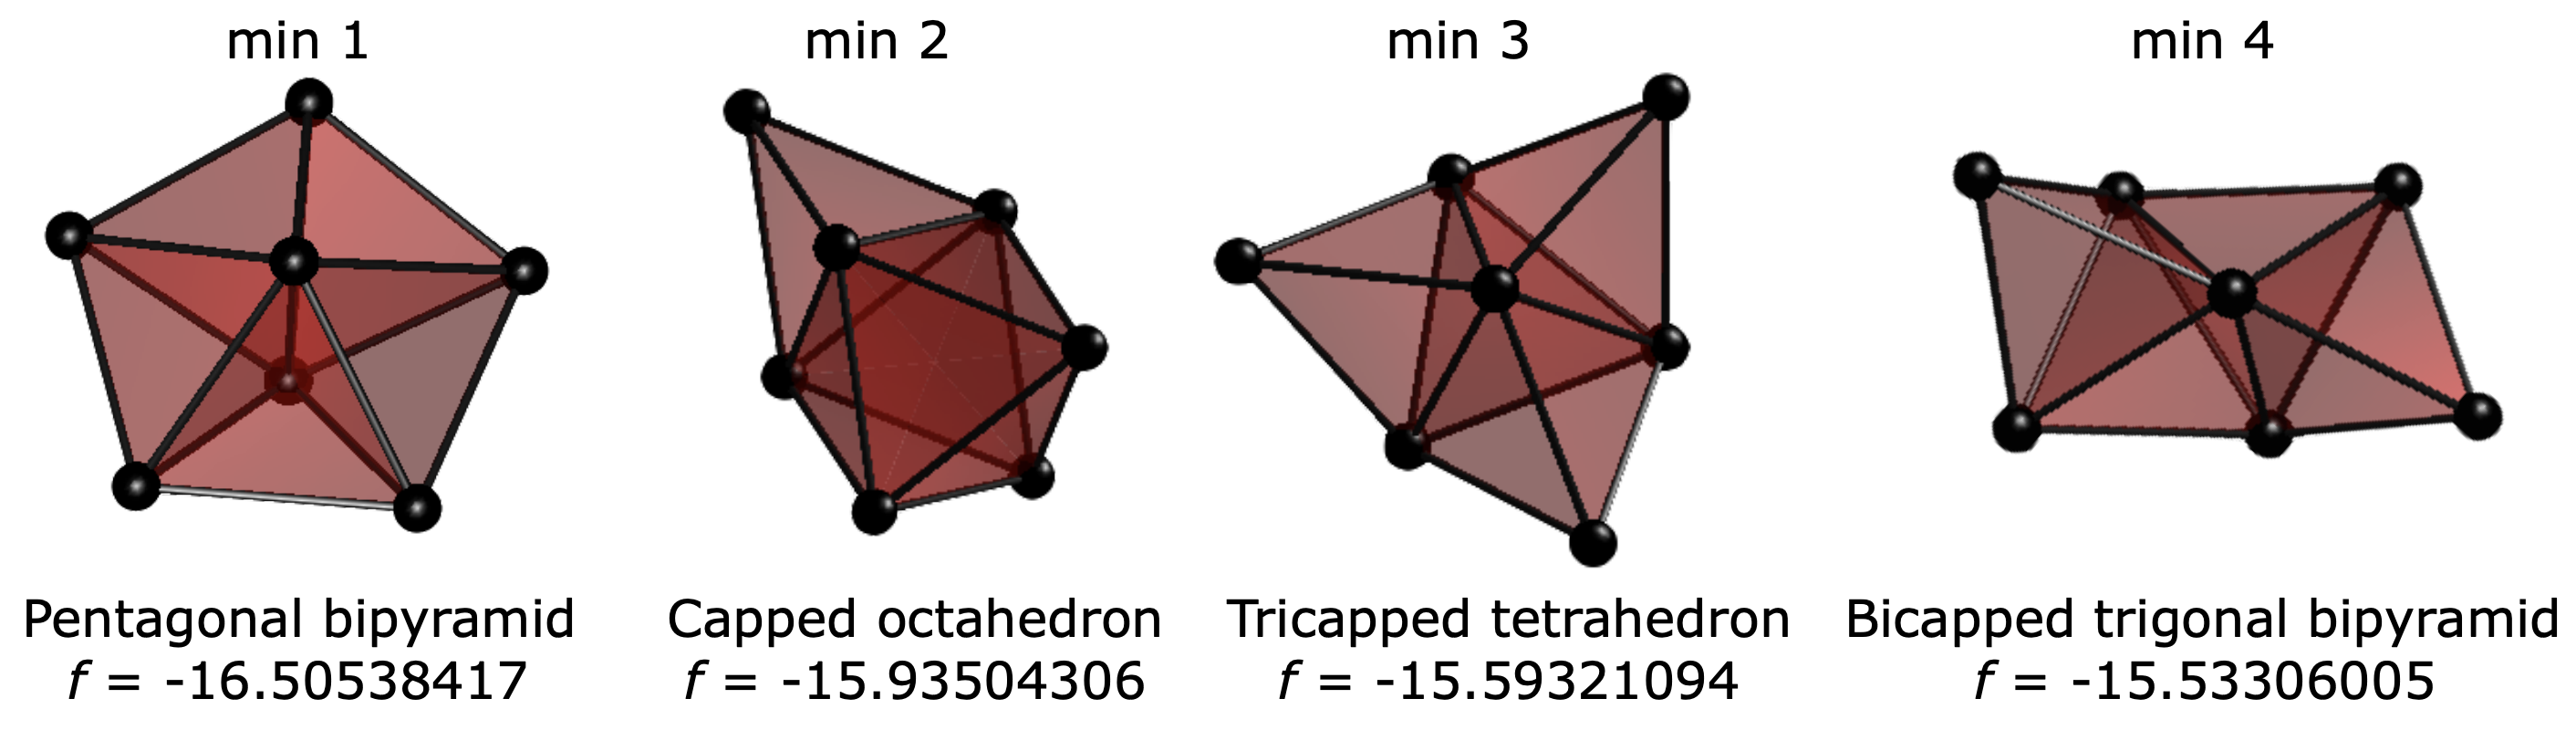
\includegraphics[scale=0.25]{minima.png}
  \end{center}
  Add the BFGS search directions to the provided Matlab or Python codes. It is recommended to reset the matrix $B_k$ in the BFGS method to the identity every $m$th step. Try $m = 5$ and $m = 20$.

  Compare the performance of the three algorithms, the steepest descent, Newton's (already encoded), and BFGS in terms of the number of iterations required to achieve convergence and by plotting the graph of $f$ and $\lVert \nabla f \rVert$ against the iteration number for each test case. Do it for each of the four initial conditions approximating the four local minima and ten random initial conditions.
  \begin{solution}
    TODO
  \end{solution}

  \question (Approx. Problem 3.1 from [NW])
  \begin{enumerate}
    \item Compute the gradient and the Hessian of the Rosenbrock function
    \begin{equation}
      \label{eq:rosenbrock}
      f(x, y) = 100(y - x^2)^2 + (1 - x)^2.
    \end{equation}
    Show that $(1, 1)$ is the only local minimizer, and that the Hessian is positive definite at it.
    \begin{solution}
      The first-order partial derivatives of the Rosenbrock function are
      \begin{equation*}
        \frac{\partial f}{\partial x} = -400x(y - x^2) - 2(1 - x) \text{ and } \frac{\partial f}{\partial y} = 200(y - x^2),
      \end{equation*}
      hence its gradient is given by
      \begin{equation*}
        \nabla f(x, y) = \begin{bmatrix} -400x(y - x^2) - 2(1 - x) \\ 200(y - x^2) \end{bmatrix}.
      \end{equation*}
      The second-order partial derivatives of the Rosenbrock function are
      \begin{equation*}
        \frac{\partial^2 f}{\partial x^2} = -400(y - x^2) + 800x^2 + 2 \text{ and } \frac{\partial^2 f}{\partial x \partial y} = -400x
      \end{equation*}
      and
      \begin{equation*}
        \frac{\partial^2 f}{\partial y \partial x} = -400x \text{ and } \frac{\partial^2 f}{\partial y^2} = 200
      \end{equation*}
      so its Hessian is
      \begin{equation*}
        \begin{bmatrix}
          -400(y - x^2) + 800x^2 + 2 & -400x \\ -400x & 200
        \end{bmatrix}.
      \end{equation*}
      TODO
    \end{solution}
    \item Program the steepest descent, Newton's, and BFGS algorithms using the backtracking line search. Use them to minimize the Rosenbrock function (\ref{eq:rosenbrock}). First start with the initial guess $(1.2, 1.2)$ and then with the more difficult one $(-1.2, 1)$. Set the initial step length $\alpha_0 = 1$ and plot the step length $\alpha_k$ versus $k$ for each of the methods.

    Plot the level sets of the Rosenbrock function using the command \texttt{contour} and plot the iterations for each method over it.

    Plot $\lVert (x_k, y_k) - (x^*, y^*) \rVert$ versus $k$ in the logarithmic scale along the $y$-axis for each method. Do you observe a superlinear convergence? Compare the performance of the methods.
    \begin{solution}
      TODO
    \end{solution}
  \end{enumerate}
\end{questions}

\end{document}
